%\documentclass[masters]{undergraduate-thesis}
\documentclass[bachelors]{undergraduate-thesis} % use this line if you are writing a bachelor's thesis

%% Packages. All ducumentation is on the web, google for package name + latex
\usepackage{subfiles}
\usepackage{hyperref}
\usepackage{babel}
\usepackage{csquotes}
\usepackage[giveninits=true,
            uniquename=init,
            style=apa,
            backend=biber,
            apabackref=true,
            abbreviate=false,
            maxbibnames=99,
            ]{biblatex}
\usepackage{mathtools}
\usepackage{tikz}
\usepackage{pgfplots}
\usepackage{subfig}
\usepackage{float}
\usepackage[capitalise,noabbrev]{cleveref}
\usepackage{pdfpages}
\usepackage[detect-all]{siunitx}
\usepackage[intoc]{nomencl}
\usepackage[acronym,xindy,toc]{glossaries}
\usepackage{etoolbox}
\usepackage{multicol}

% set multicolumn spacing for nomenclature
\setlength{\columnsep}{1cm}

% no page breakt in notation section
\renewcommand*{\glsclearpage}{}

% nomenclature
\makenomenclature

% glossaries
\makeglossaries

% pgfplots
\pgfplotsset{compat=newest}
\usepgfplotslibrary{units}

% required for apa-style
\DeclareLanguageMapping{swedish}{swedish-apa}
\DeclareLanguageMapping{english}{english-apa}

% Reference section titles in English and Swedish
\DefineBibliographyStrings{english}{%
	bibliography = {References},
}
\DefineBibliographyStrings{swedish}{%
	bibliography = {Referenser},
}

%% Add reference sourse file
\addbibresource{references.bib}
	

% User commands
\title{Some Title}
\subtitle{some subtitle} % Optional
\author{Gudjón Ólafur Gudjónsson \and Jón Grétar Höskuldsson} 
\thesisin{Civilingenjörsprogrammet}
\department{Department of Civil and Environmental Engineering}
\division{Division of Structural Engineering}
\researchgroup{Concrete Structures}
\reportno{201X:XX} % contact your examiner for report number
\copyrightyear{201X}
\keywords{Permanent Diaphragm Walls, Diaphragm Walls, Functional Requirements}


% You should scale the figure according to textwidth and or paperheight.
\coverfigure{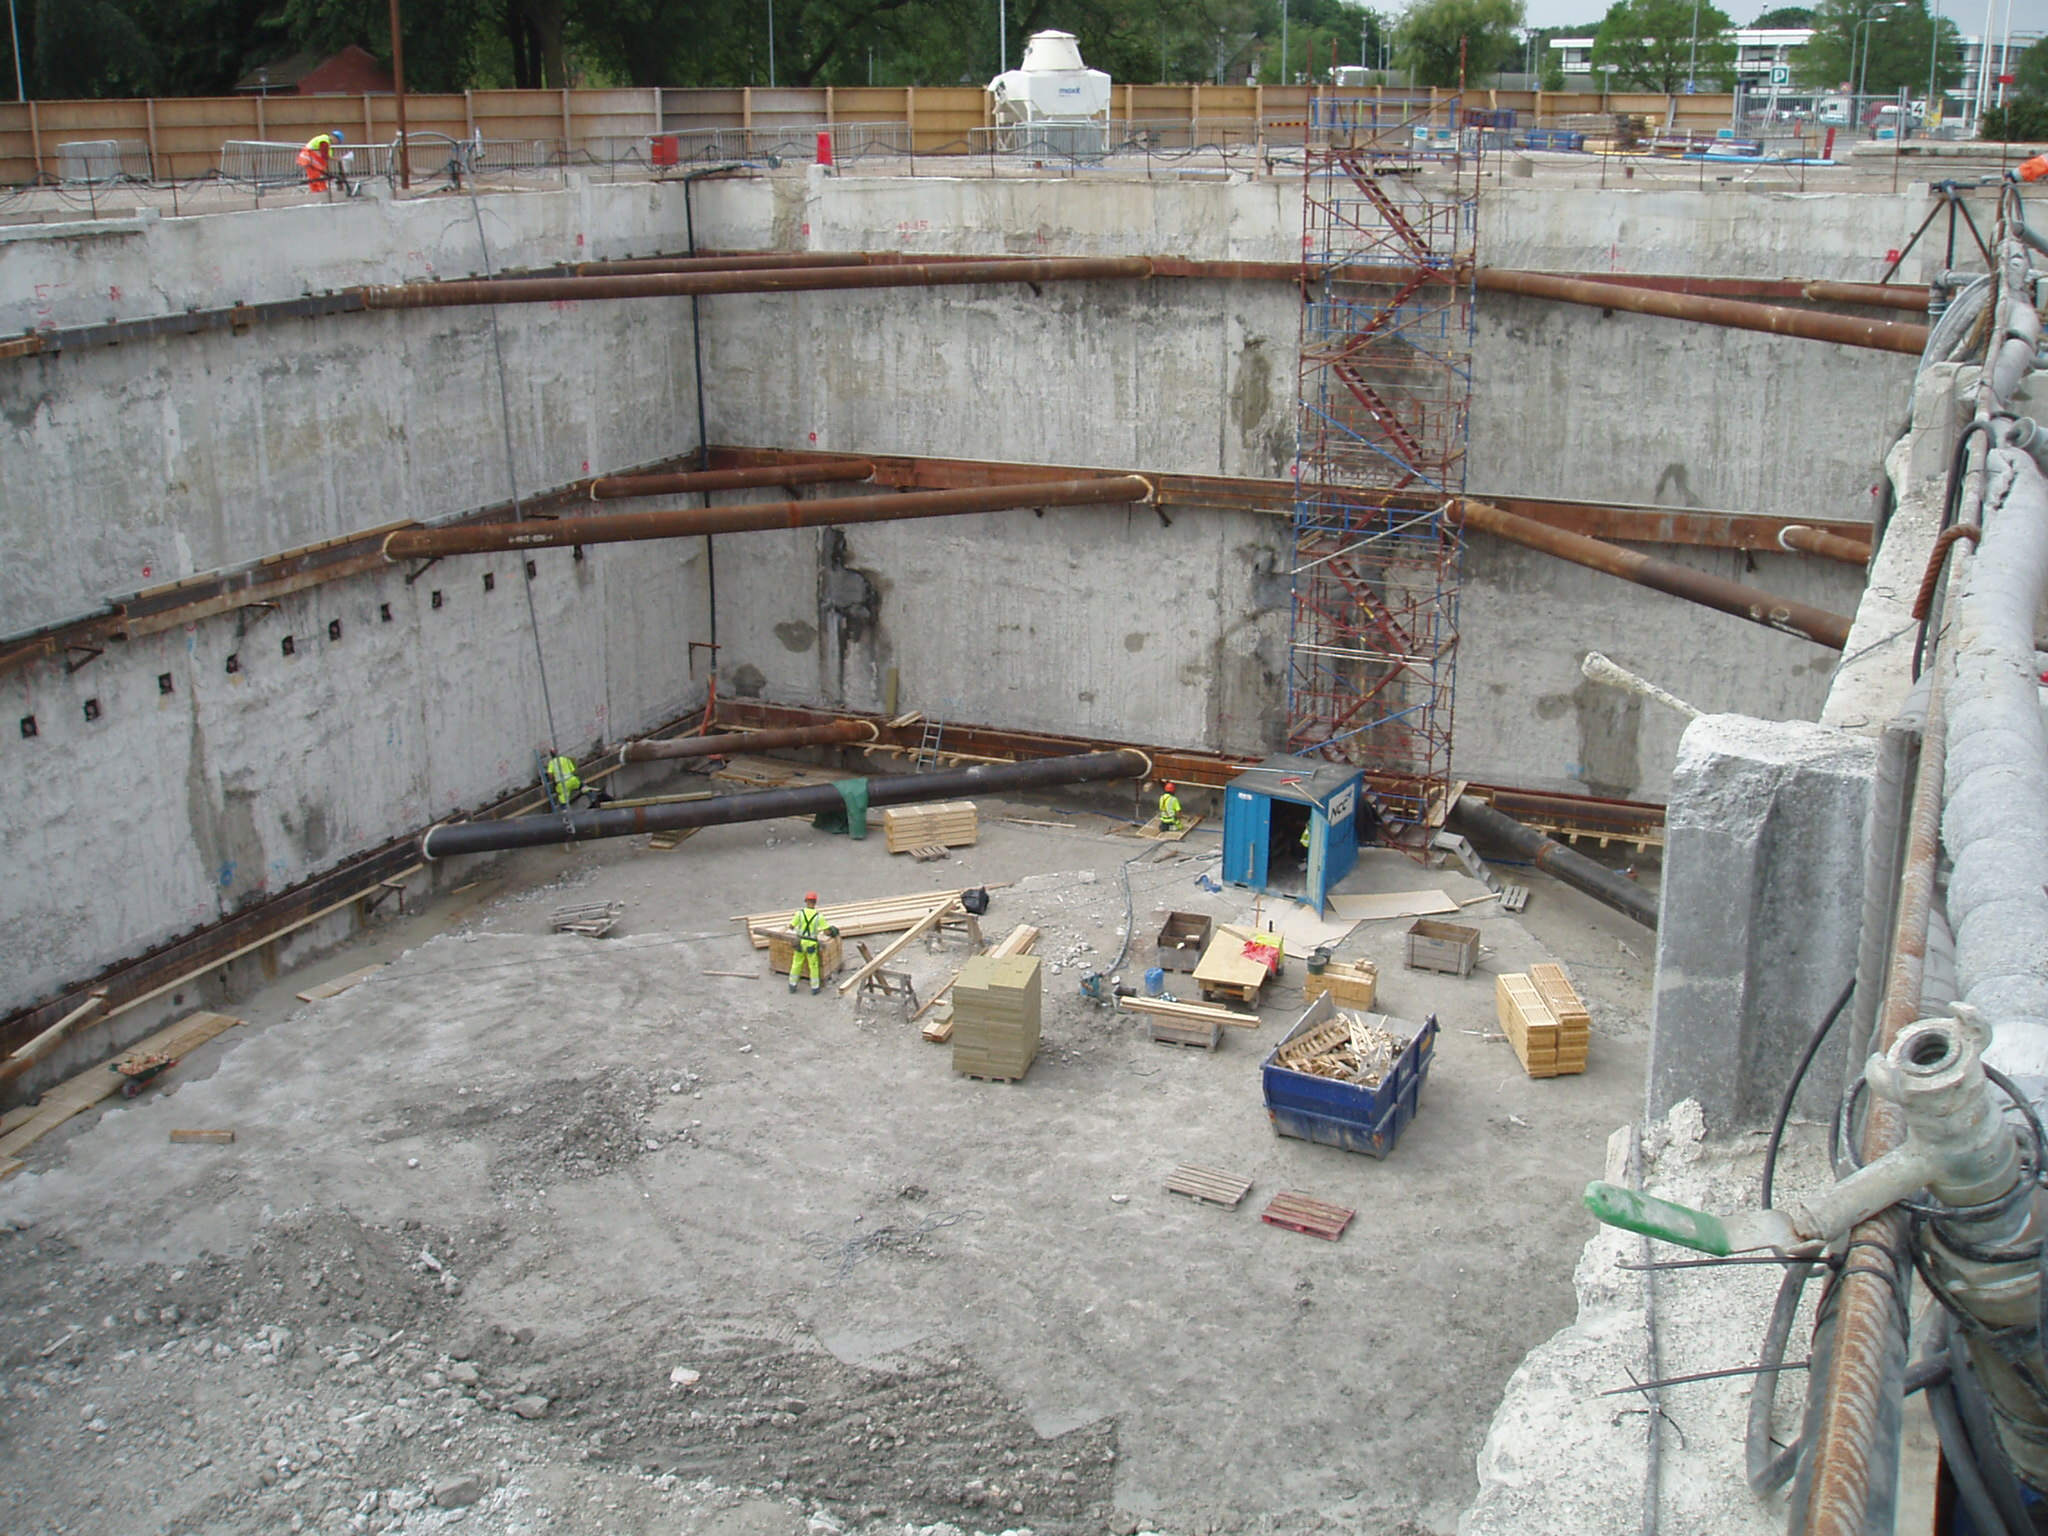
\includegraphics[width=\textwidth,height=0.37\paperheight,keepaspectratio]{img/P6290037.JPG}}
\covercaption{City Tunnel Diaphragm Walls, TEMP pic}

% optional
\colophon{%
The thesis was created using \LaTeXe{} and \texttt{biblatex} and edited on \texttt{www.sharelatex.com}. The typesetting software was the \TeX{} Live distribution. The text is set in Times New Roman. Graphs were creating using {\scshape pgfplots} and MS Excel. Figures were created using {\scshape inkscape}.
}

\firstabstract{%
Here goes the text for the Abstract
}


\preface{%
Here goes the text for the Preface.
}

% secondary language
% You only need to use this if you (1) are writing a bachelor thesis in Swedish which should have an English abstract, or (2) if you are writing a Master's thesis and want to include a Swedish abstract (which is optional).
\secondarylanguage{english}
\thesisinsecondlang{Building and Civil Engineering}
\titlesecondlang{Some Title secondary language}
\subtitlesecondlang{some subtitle secondary language} % Optional
\keywordssecondlang{keywords in, secondary, language}
\departmentsecondlang{Department's name in secondary language}
\divisionsecondlang{Division's name in secondary language} % Optional
\researchgroupsecondlang{Research group's name secondary language} % Optional
\abstractsecondlang{%
	This is the abstract text in the secondary language
}


\begin{document}
\maketitle
% Here goes the content of your thesis. 
\chapter{Introduction}
This is a template!

\section{Background}
Write about the thesis background here.
\section{Problem description}
This is where you describe you problem.
\section{General aim}
By now you know what to do here :)
\section{Method / Outline }
...

\section{Objectives}
...

\section{References}
Your reference data should be contained in \texttt{references.bib}. Open the file using a text editor and look at its content. Your own references need to have the same structure! You cite a reference in these ways:
\begin{itemize}
	\item \parencite[pre note][post note]{Harryson2014}
	\item \textcite[][Chapter~2]{Noren2006}
	\item \cite{Harryson2014}
	\item \citeauthor{Harryson2014}
	\item \citetitle{Harryson2014}
	\item \cite{box1978,Harryson2014,matlab}
	\item \textcite{LectureA}
\end{itemize}

\section{Cross-references}
Cross-references within your own thesis are taken care of by the package \texttt{cleverref}. Making a cross-reference to a figure is done in this way: \cref{figure:test} (the name in the curly brackets could be anything).

\section{Equations}
Here is how to typeset equations in \LaTeX{}.

\begin{align}
\sigma = E\varepsilon \label{coolequation}
\end{align}
and here is how to align several equations using the \& symbol:
\begin{align}
A &= Bx \\ % double backslash to break to a new line
c + D +\frac{2}{\phi} &= \sqrt{B}
\end{align}
and here is how to suppress numbering of equations
\begin{align*}
\sigma = E\varepsilon
\end{align*}
and this is how to cross-reference to an equation: \cref{coolequation}.

\subsection{In-line math}
Use the \$-symbol to typeset in-line math like so: $\sigma = E\varepsilon$. This important because in-line math should be italicized. For example, if you want to write the symbol for Young's modulus, it needs to be done in this way: $E$, not: E. If the letter ``E'' is italicized, then it is a physical quantity, namely Young's modulus, whereas a normal ``E'' is just an E.

\subsection{Acronymes}
Define you acronymes in \texttt{notation.tex}. \acrlong{fem}, \acrshort{fem}, \acrfull{fem}.

\subsection{Glossaries}
A glossaries can be useful to include for words that the reader is assumed to have no prior knowledge of. You define your glossaries in \texttt{notation.tex} and the reference to them like this: \Gls{polyhedron}, \gls{polyhedron} and \glspl{polyhedron}.
\chapter{Units}
Units are typeset using the package \texttt{siunitx}. Most numerical values you will typeset have units, except e.g. strain. Here are two examples of badly typeset units: 
\begin{align*}
\sigma &= 100 mpa \\
\sigma &= 100\, Mpa
\end{align*}

The correct way looks like this:
\begin{align*}
\sigma = \SI{100}{\mega\pascal}
\end{align*}
The unit should \emph{not} be italicized and should have a correct spacing between its numerical value. This is automatically taken care of by the package \texttt{siunitx}. Common units are typeset in this way: $\SI{10}{\meter\squared}$, $\SI{10e-5}{\meter\cubed}$, $\SI{10}{\kilo\newton}$ and $\SI{10}{\gram\per\meter\squared\per\second}$. The number goes in the first pair of curly brackets, and the unit in the second pair. Typesetting units \emph{without} numerical value is done in this way: $\si{\kilo\newton}$.
\chapter{Section headings}
Here is how you subdivide your thesis into different levels:

\section{Section}
This is a Section

\subsection{Subsection}
This is a Subsection.

\subsubsection{Subsubsection}
This is a Subsubsection. Your should avoid levels below this one.


\chapter{Graphics}

\begin{figure}[H]
\centering
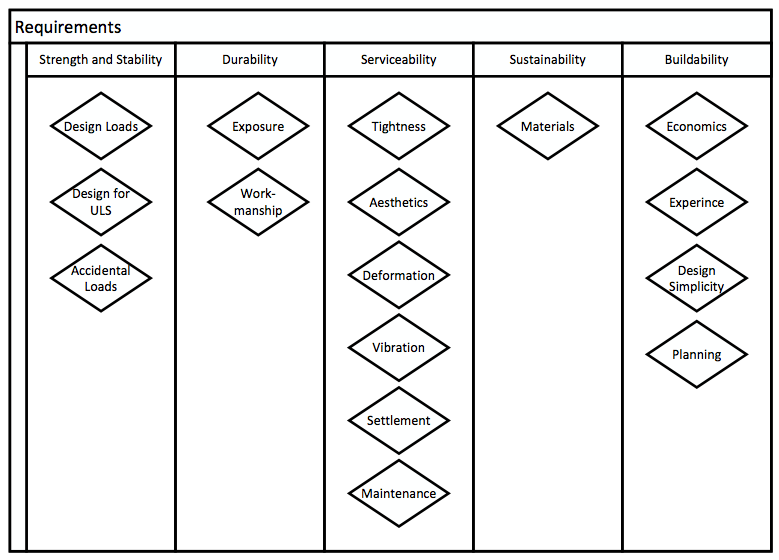
\includegraphics[scale=0.4]{figures/GR-FR.png}
\caption{Functional requirements for Buildability.}
\label{figure:test}
\end{figure}

bla bla bla....

\section{Plots}
Plots are preferably done using the package \texttt{pgfplots}. Below is an example given. The example also show how to put figures side-by-side in your document using the \texttt{\textbackslash subfloat} command. Open \texttt{data.txt} in a text editor and have a look at its structure. The \LaTeX{} document reads the data from the text file and produces a plot. Axes are automatically scaled depending on the data range given in the text file. 

%------------------------------------------------------------------------------------
\begin{figure}[H]
\centering
\subfloat[Diagonal components of $\bar{D}$.]{
\begin{tikzpicture}
\begin{axis}[
	scale=0.85, % size of the plot
	every axis/.append style={line width=1pt},
    xlabel = $\bar{\varepsilon}_\text{zz}$,
    ylabel style={align=center},
    ylabel = $(\bar{D})_\bullet/D_\text{cp}$,
    y unit = -,
    x unit = -,
    cycle list name=linestyles,
    legend style={cells={anchor=west}},
    legend pos=north west,
    ]
\addplot table[mark=none,x expr=\thisrow{strain},y expr=\thisrow{Dxx}] {datafiles/data.txt};
\addplot table[mark=none,x expr=\thisrow{strain},y expr=\thisrow{Dyy}] {datafiles/data.txt};
\addplot table[mark=none,x expr=\thisrow{strain},y expr=\thisrow{Dzz}] {datafiles/data.txt};
\legend{$(\bar{D})_{xx}$,$(D)_{yy}$,$(D)_{zz}$};
\end{axis}
\end{tikzpicture}
\label{fig:a}
}\hfill % \hfill fills out the space inbetween the plots
\subfloat[Off-diagonal components of $\bar{D}$.]{
\begin{tikzpicture}
\begin{axis}[
	scale=0.85,
	every axis/.append style={line width=1pt},
    xlabel = $\bar{\varepsilon}_\text{zz}$,
    ylabel style={align=center},
    ylabel = $(\bar{D})_\bullet/D_\text{cp}$,
    ylabel style={yshift=-0.2cm},
    y unit = -,
    x unit = -,
    cycle list name=linestyles,
    legend style={cells={anchor=west}},
    legend pos=north west,
    ]
\addplot table[mark=none,x expr=\thisrow{strain},y expr=\thisrow{Dxy}] {datafiles/data.txt};
\addplot table[mark=none,x expr=\thisrow{strain},y expr=\thisrow{Dxz}] {datafiles/data.txt};
\addplot table[mark=none,x expr=\thisrow{strain},y expr=\thisrow{Dyz}] {datafiles/data.txt};
\legend{$(D)_{xy}$,$(\bar{D})_{xz}$,$(\bar{D})_{yz}$};
\end{axis}
\end{tikzpicture}
\label{thelabelcanbeanyingreally}
}
\caption{Components of the macroscale diffusivity tensor, $\bar{D}$, as a function of macroscale strain. Numerical values are normalized with respect to $D_\text{cp}$.}
\label{omg}
\end{figure}
%------------------------------------------------------------------------------------
You can cross-reference to each of the figures in this way: \cref{fig:a} and \cref{thelabelcanbeanyingreally}. You can also plot analytical functions \texttt{pgfplots} as shown in \cref{analytical} below.
%------------------------------------------------------------------------------------
\begin{figure}[H]
\centering
\begin{tikzpicture}
\begin{axis}[legend pos= north west]
\addplot[dashed,domain=-1:1]{x^2};
\addplot[dotted,thick,domain=1:2]{x^2 + sqrt(x)};
\legend{$x^2$,$x^2 + \sqrt{x}$}
\end{axis}
\end{tikzpicture}
\caption{Examples of analytical functions.}
\label{analytical}
\end{figure}
%------------------------------------------------------------------------------------


% references
\cleardoublepage
\printbibliography[heading=bibintoc]

% appendicies
\cleardoublepage
\begin{appendices}
\chapter{Your first Appendix}
The contents of your appendicies go here.
\chapter{Your second Appendix}
The contents of your appendicies go here.

\chapter{Your third Appendix}
If you want to append separate PDFs, you can do it in this way. Note that the page footer (including page numbering) is superiposed in the apppended PDF.

\includepdf[pages=-,pagecommand=\thispagestyle{fancy}]{appendedPDFs/appended-pdf.pdf}
\end{appendices}
\end{document}

 
